\chapter{Phylogenetic Bayesian models}
\minitoc
\label{sec:phylo_bayes}

\section{Probability of the data}

\subsection{Probability of transitions for a branch}



\subsection{Probability of transitions for a tree}
\begin{figure}[thbp]
	\begin{center}
		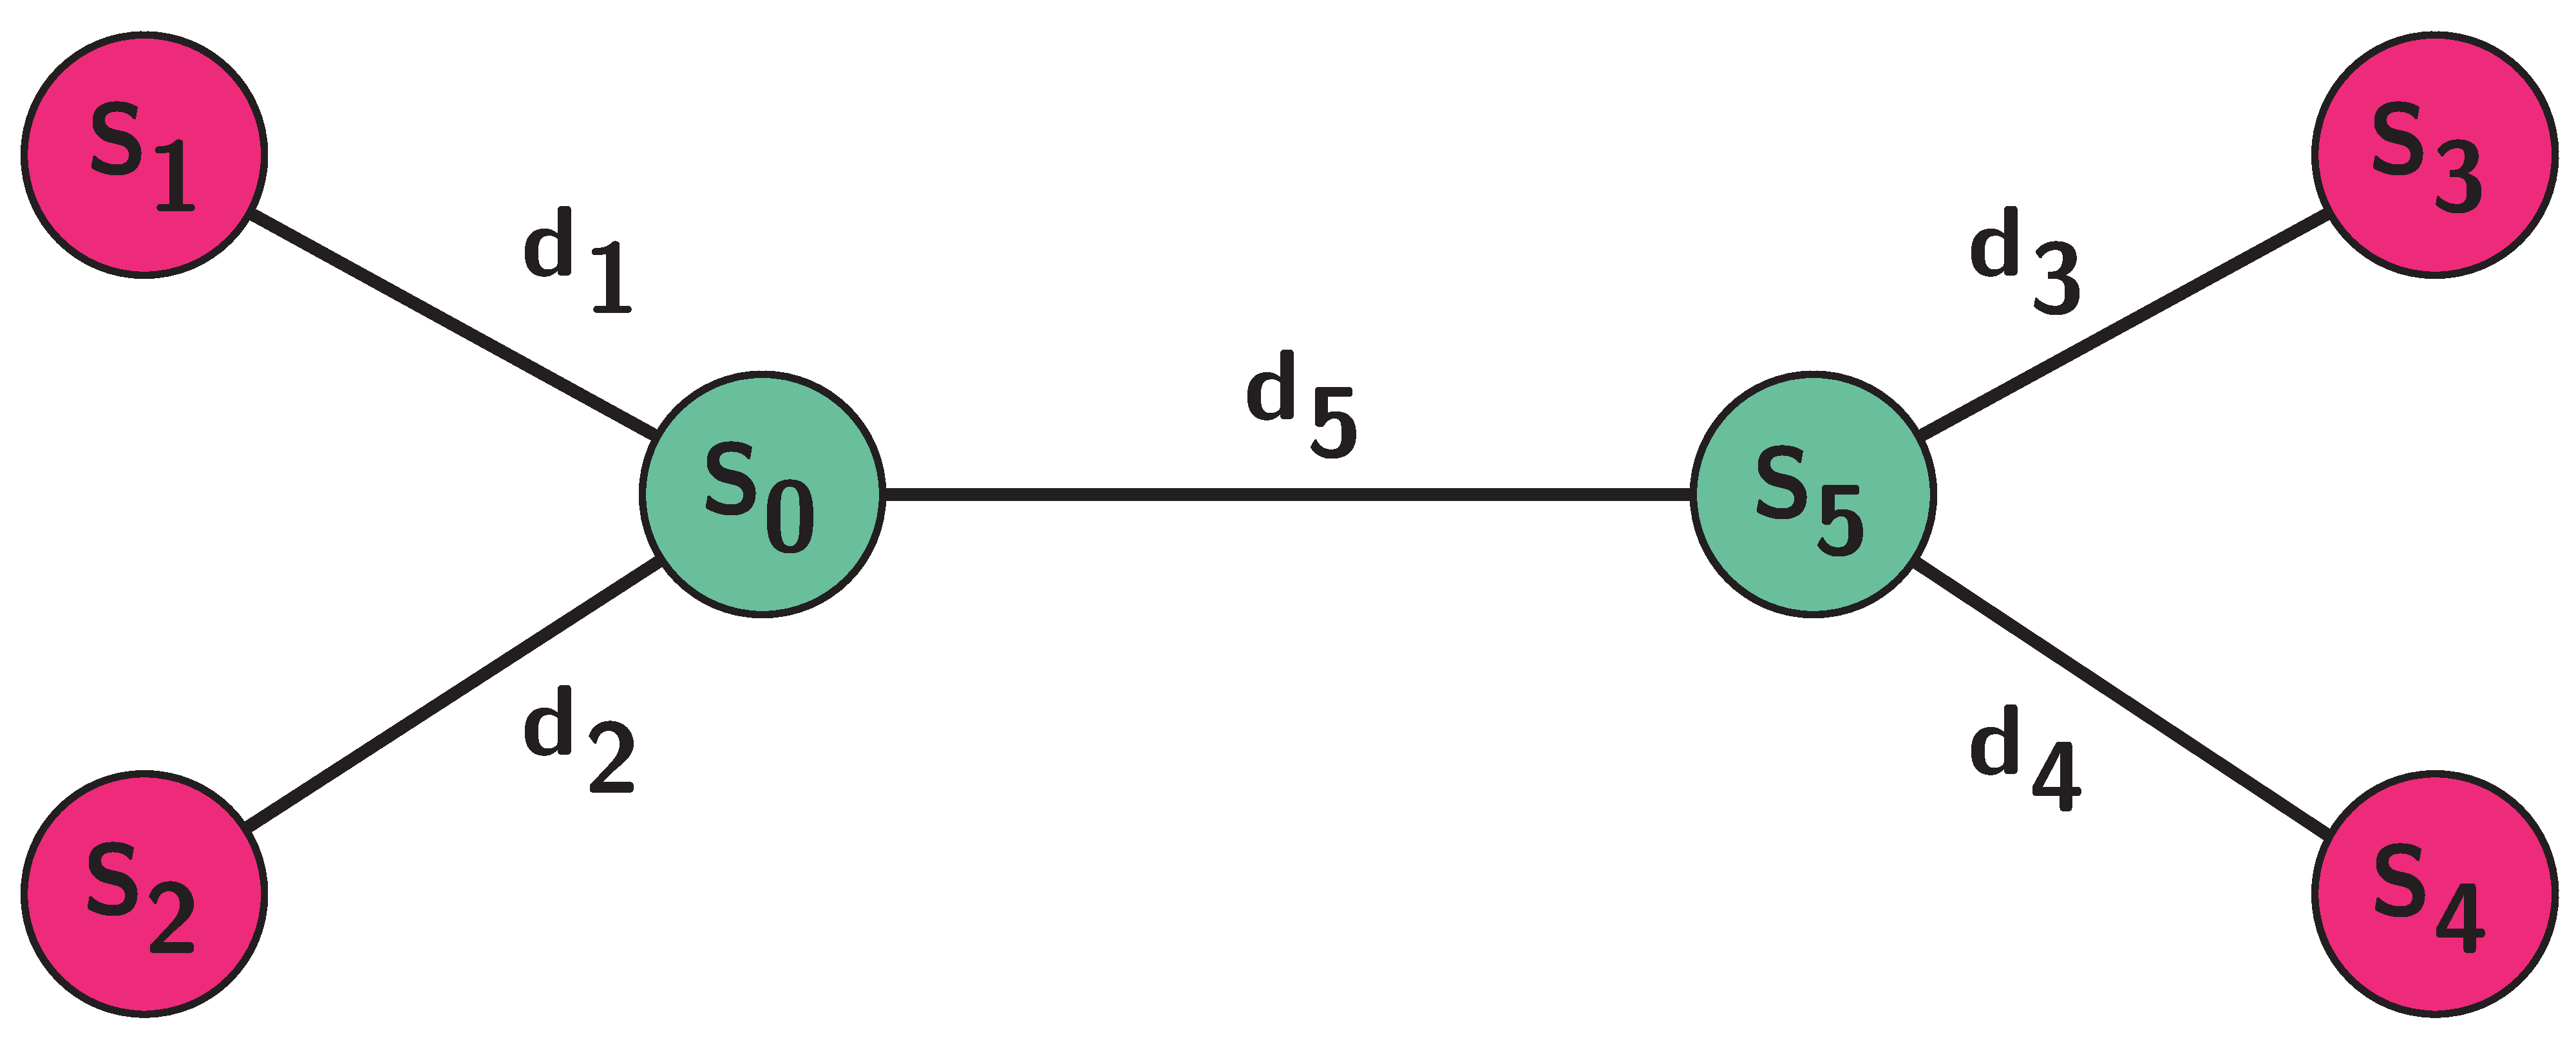
\includegraphics[width=\textwidth] {figures/pruning}
	\end{center}
	\caption{Likelihood computation of a tree}
\end{figure}

\begin{itemize}
	\item $\tau$ is the tree with given branch lengths ($d_i$).
	\item $\mu$ is mutation matrix ($4\mathrm{x}4$).
	\item $\bm{F}^{k}$ is the fitness vector ($1\mathrm{x}20$) of amino-acids at site $k$.
	\item $\Data=\{\si, \sii, \siii, \siiii \}$ is the observed data at the leaves, at site $k$.
	\item $\s$ and $\siiiii$ are the states of the internal nodes (assumed known), at site $k$.
\end{itemize}  
Likelihood of the data, at site $k$, given the states of the internal nodes is:
\begin{equation*}
P\left(\Data| \tau, \mu, \bm{F}^{k}, \s, \siiiii \right) = P_{\s \si}(d_1) \cdot P_{\s \sii}(d_2) \cdot P_{\s \siiiii}(d_5) \cdot P_{\siiiii \siii}(d_3) \cdot P_{\siiiii \siiii}(d_4)
\end{equation*}
Likelihood of the data at site $k$, given all possible states of internal node is:
\begin{equation*}
P\left(\Data| \tau, \mu, \bm{F}^{k}\right) = \sum_{\s=1}^{61}  \sum_{\siiiii=1}^{61} \pi(\s) \cdot P_{\s \si}(d_1) \cdot P_{\s \sii}(d_2) \cdot P_{\s \siiiii}(d_5) \cdot P_{\siiiii \siii}(d_3) \cdot P_{\siiiii \siiii}(d_4) 
\end{equation*}

\subsection{Pruning algorithm}

For an inner node $i$ with offspring $o_1$ and $o_2$, $L_{i} \left( \sn, \tau, \mu, \bm{F}^{k} \right)$ is defined recursively as:
\begin{equation*}
L_{i} \left( \sn, \tau, \mu, \bm{F}^{k} \right) = \left[ \sum_{x=1}^{61} P_{\sn x }(d_{o_1}) L_{o_1}\left( x, \tau, \mu, \bm{F}^{k} \right) \right] \cdot \left[ \sum_{x=1}^{61} P_{\sn x }(d_{o_2}) L_{o_2}\left( x, \tau, \mu, \bm{F}^{k} \right) \right]
\end{equation*}
\begin{figure}[thbp]
	\begin{center}
		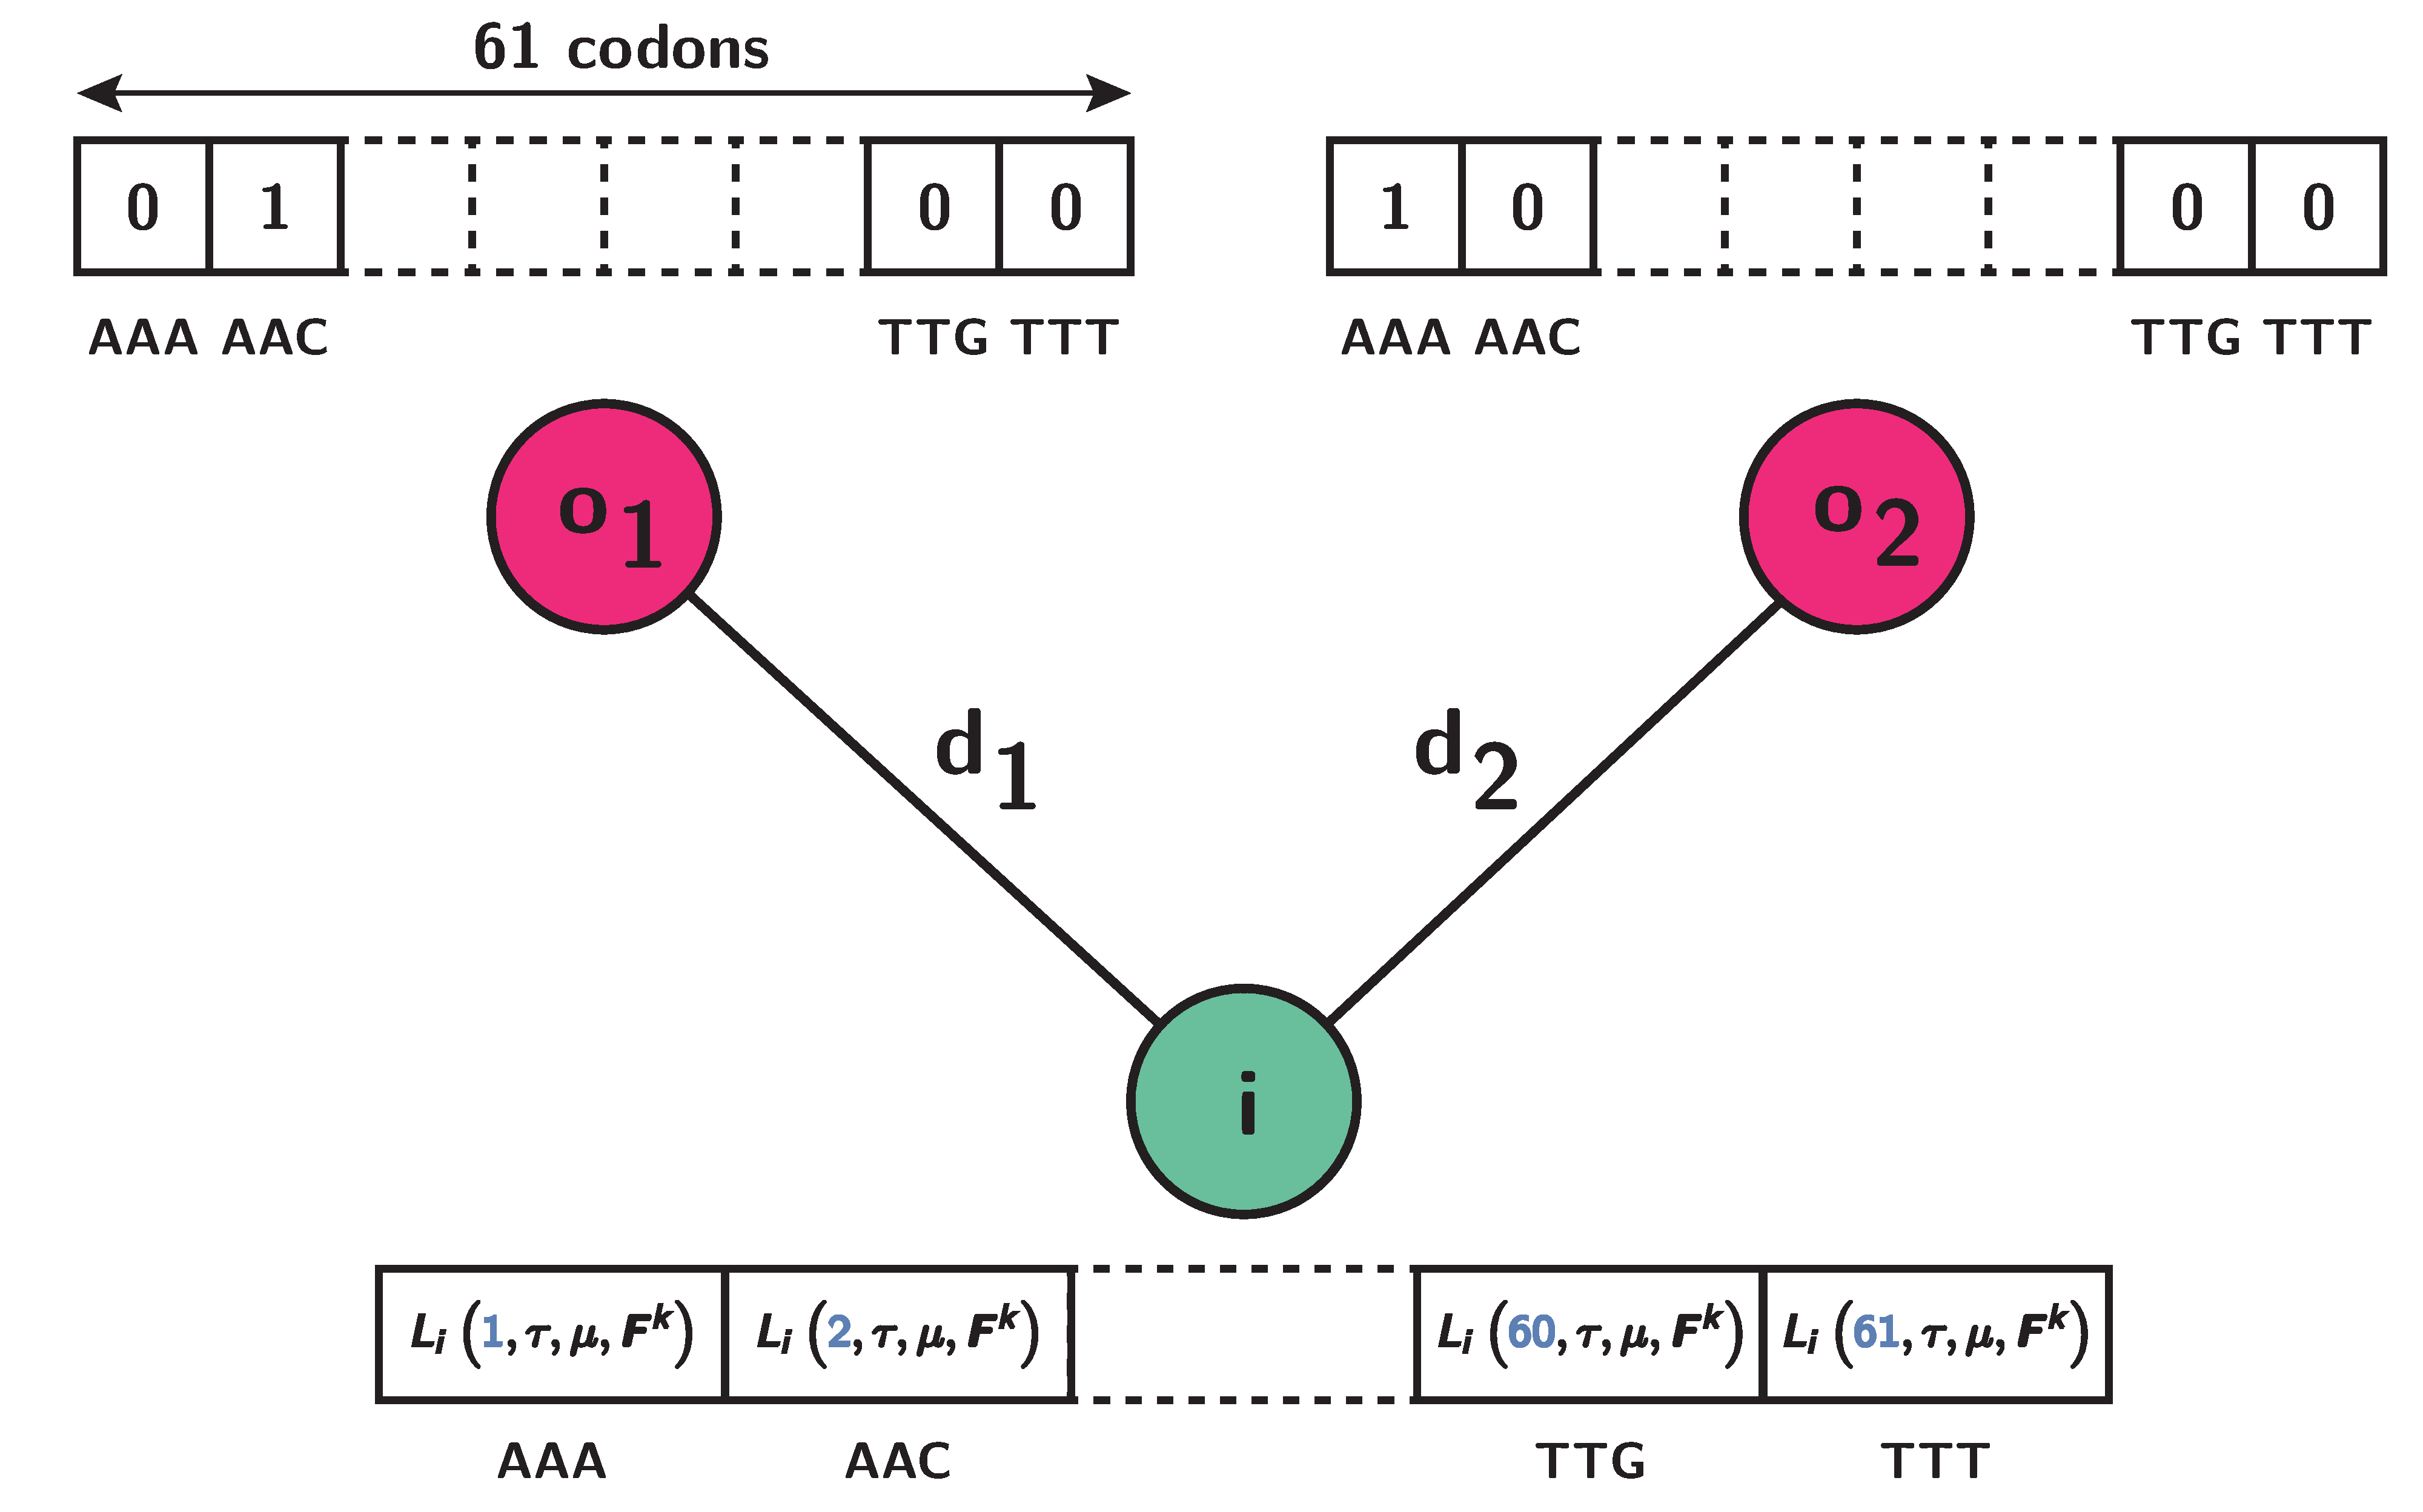
\includegraphics[width=\textwidth] {figures/pruning-children}
	\end{center}
	\caption{Formula of pruning algorithm at an inner node}
\end{figure}

And for a leaf $i$:
\begin{equation*}
L_{i}\left( \sn, \tau, \mu, \bm{F}^{k}\right) =
\begin{dcases}
1, & \text{if } \sn = {\color{PINK}{S_i^{k}}} \\
0, & \text{otherwise.}
\end{dcases}
\end{equation*}

Then the likelihood of the data at site $k$, given all possible states of internal node is:
\begin{equation*}
P\left(\Data| \tau, \mu, \bm{F}^{k}\right) = \sum_{x=1}^{61} \pi(x) L_{\text{root}} \left( x | \tau, \mu, \bm{F}^{k} \right)
\end{equation*}

\begin{figure}[thbp]
	\begin{center}
		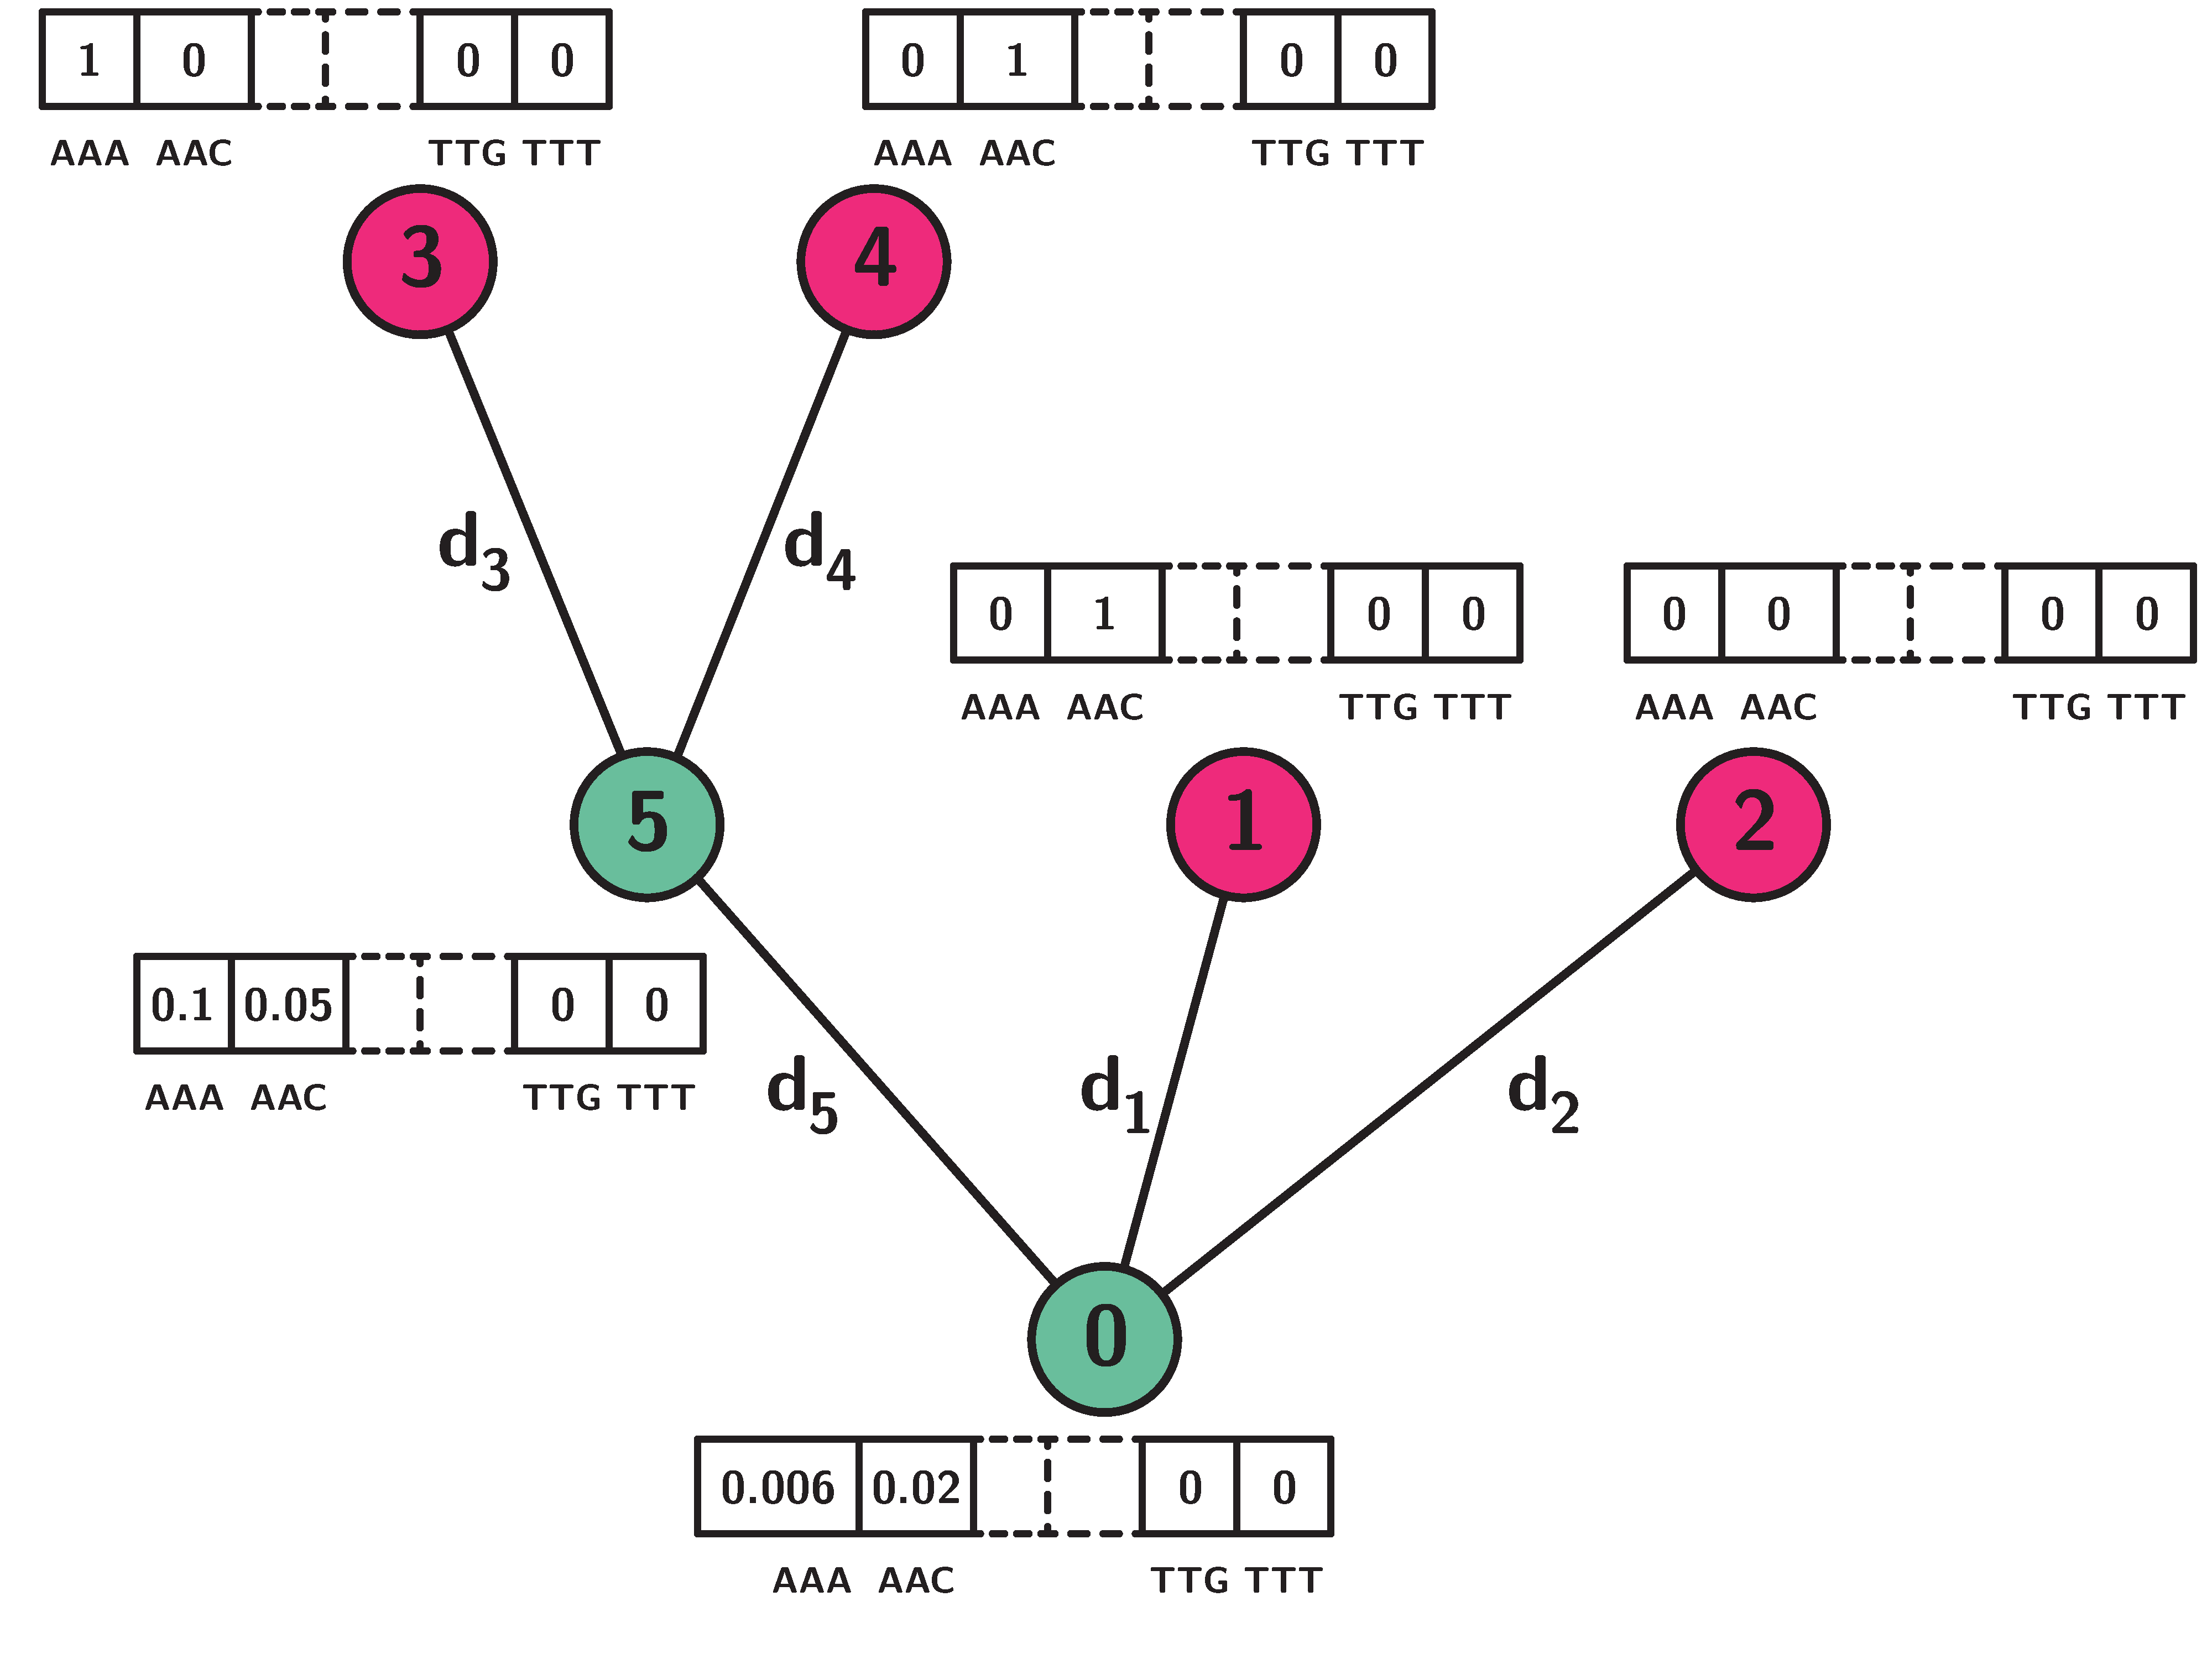
\includegraphics[width=\textwidth] {figures/pruning-algo}
	\end{center}
	\caption{Recursive formula for pruning algorithm}
\end{figure}

\section{Maximum likelihood estimation}
For a statistician this is the easiest of the methods to
understand. A parametric model $({\bf \theta},T)$ is posulated,
$\theta$ is a $\eta$-dimensional vector that we explain below and
${\cal T}$ is the tree's topology.
Under this model
the likelihood for each possible tree ${\cal T}$ is separately computed for
each character or site, the independence of sites then allows the total
likelihood of the tree for all data 
to be computed
by taking the product.

The first part of the vector
of parameters ${\bf \theta}$ comes from
the substitution model as explained above.
The number of other parameters that have
to be specified depends on the complexity of the model.
If a molecular clock \footnote{branch lengths in evolutionary
	change
	depend linearly on time} is  postulated,
speciation times $\{t_1,t_2,...t_{N-2} \}$ (splitting events)
are the other parameters.
Otherwise both
the branch lengths $\{v_1,v_2,...v_{N-2} \}$
and the different
rates 
along those branches have to be parametrized.

The substitution parameters are estimated from the data.
A complete model including distributions of
separation events is postulated and the likelihood can be computed
for each possible tree by computing the likelihood of the tree
given each site $X_{.j}$
$$f(X_{.j}|\theta_1,\theta_2,\ldots,\theta_{\eta},{\cal T})$$
This actually requires computing the likelihood of all the
subtrees, so the method is recursive.
$${\cal L}(\theta_1,\theta_2,\ldots,\theta_{\eta}|X_{.1},X_{.2},\ldots,X_{.k},{\cal T})
=\prod_{j=1}^k f(X_{.j}|\theta,{\cal T}) $$

As the assumptions are  essential,
I present them here:
\begin{itemize}
	\item Each site in the sequence evolves independently.
	\item Different lineages evolve independently.
	\item Each site undergoes substitution at an expected rate which  is  chosen from  a  series  of  rates with a given distribution.
\end{itemize}
Fancier versions of the procedure enable
different sites to have different
evolution rates.

\section{Bayesian estimation}

The Bayesian Paradigm can be seen in some
ways as an extra step in the modelling world just
as parametric modelling is. We have seen how we
could use probabilistic models to infer about 
some unknown aspect either by confidence intervals
or by hypothesis testing.

The motivation for any statistical analyses
is that some ``target population'' is not well understood- some
aspects of it are unknown or unsure.

The idea in this paradigm is to say
that any uncertainty can be modelled
in a probabilistic way.

It is true that there are very rarely situations when one doesn't
know anything at all, asked to measure the table,
you won't want to use a ``pied de coulisse''(callipers) or a 
100 yard measuring ribbon. 

The probability model that we build can be quite approximate,
it reflects one's beliefs and any prior experience
we may have, it is described as personal or subjective.

Why ? Because it is different from person to person, examples
that are easy to understand are about horse betting,
the stock exchange...

So when the uncertainty about the model can be boiled down
to a parameter $\theta$ the Bayesian statistician treats $\theta$ as if
it were a random variable $\Theta$ whose distribution describes that 
uncertainty.

Elliciting a whole distribution may seem a challenge,
in fact it's done by successive events of the type $\Theta \leq \theta$,
and does NOT have to be very precise.

A subjective/personal probability is going to be
subject to modification upon acquisition of
further information supplied
by experimanetal data.

Suppose a distribution with density $g(\theta)$ describes one's
present uncertainties about some probability model 
with density $f(x|\theta)$.

Those uncertainties will change with the acquisition of data 
obtained by doing the experiment modelled by $f$.

Bayes theorem is essential in updating :
$$P(H|data)=\frac{P(data|H)P(H)}{P(data)}$$

The probability of H given the data is called the posterior
probability of H, it is posterior to the data.
The unconditional probability of $H$ : $P(H)$ is the prior
probability of H.

For given data $P(data|H)$ is the likelihood of H.

For given data we often write :
$$P(H|data) \propto P(data|H) P(H)$$
The posterior is proportional to the likelihood time the prior.

\subsection{Monte-Carlo Markov-Chain}

\subsection{Metropolis-Hastings}

\subsection{Gibbs sampling}

\subsection{Data augmentation}

